\documentclass[11pt]{article}

\usepackage[letterpaper,margin=0.82in,headheight=15pt]{geometry}
\usepackage[T1]{fontenc}
\usepackage[utf8]{inputenc}
\usepackage{lmodern}
\usepackage{microtype}
\usepackage{graphicx}
\usepackage{booktabs}
\usepackage{siunitx}
\usepackage{xcolor}
\usepackage{hyperref}
\usepackage{fancyhdr}
\usepackage{titlesec}
\usepackage{caption}
\usepackage{enumitem}
\usepackage{float}
\usepackage{placeins}

\definecolor{navy}{HTML}{17365D}
\definecolor{blue}{HTML}{2E75B6}
\definecolor{lightblue}{HTML}{D9EAF7}
\definecolor{orange}{HTML}{D55E00}
\definecolor{graytext}{HTML}{555555}

\hypersetup{
  colorlinks=true,
  linkcolor=navy,
  urlcolor=blue,
  pdftitle={Concise Building Vibration Assessment},
  pdfsubject={Peak-centered comparison of candidate laboratory spaces}
}
\graphicspath{{../figures/}}
\sisetup{
  scientific-notation=true,
  round-mode=figures,
  round-precision=3,
  exponent-product=\times,
  detect-all
}
\DeclareSIUnit{\sqrthertz}{\hertz\tothe{0.5}}
\newcommand{\asdunit}{\si{\meter\per\second\squared\per\sqrthertz}}
\newcommand{\freq}[1]{\SI[scientific-notation=false]{#1}{\hertz}}
\newcommand{\freqrange}[2]{\SIrange[scientific-notation=false]{#1}{#2}{\hertz}}

\pagestyle{fancy}
\fancyhf{}
\lhead{\textcolor{graytext}{Concise Building Vibration Assessment}}
\rhead{\textcolor{graytext}{Physics Laboratories}}
\cfoot{\thepage}
\renewcommand{\headrulewidth}{0.4pt}

\titleformat{\section}{\Large\bfseries\color{navy}}{\thesection}{0.7em}{}
\titleformat{\subsection}{\large\bfseries\color{blue}}{\thesubsection}{0.7em}{}
\captionsetup{font=small,labelfont=bf}
\setlist{nosep,leftmargin=1.5em}
\setlength{\parindent}{0pt}
\setlength{\parskip}{0.55em}
\renewcommand{\arraystretch}{1.15}

\begin{document}

\hypersetup{pageanchor=false}
\begin{titlepage}
  \centering
  \vspace*{1.35in}
  {\color{navy}\rule{\textwidth}{1.2pt}\par}
  \vspace{0.42in}
  {\Huge\bfseries Concise Building Vibration Assessment\par}
  \vspace{0.18in}
  {\Large A peak-centered comparison for spectroscopy and other vibration-sensitive work\par}
  \vspace{0.42in}
  {\color{navy}\rule{\textwidth}{1.2pt}\par}
  \vfill
  \begin{tabular}{rl}
    \textbf{Source workbook:} & \texttt{FinalReportData.xlsx}\\
    \textbf{Measurements:} & 15 spectra from 5 measured rooms\\
    \textbf{Report date:} & July 24, 2026\\
  \end{tabular}
  \vfill
  {\large Simplified companion to the full building-vibration report\par}
\end{titlepage}
\hypersetup{pageanchor=true}
\pagenumbering{arabic}

\section{Summary}

\fcolorbox{navy}{lightblue}{%
  \begin{minipage}{0.93\linewidth}
  \textbf{\color{navy}Recommendation: use the Titan laboratory.}
  Titan has the lowest estimated broadband vibration background among the
  candidate rooms and the cleanest spectrum away from one narrow line at
  approximately \freq{29.8}. PHYS 245 is the next-best room, but it has
  more distinct peaks, especially near \freq{17.6},
  \freq{29.8}, and \freq{66.0}.
  \end{minipage}
}

For peak-sensitive spectroscopy, the important distinction is not a small
difference in the common noise floor; it is the number and size of discrete
lines. Titan's median non-mains ASD is
\SI{2.24e-4}{\meter\per\second\squared\per\sqrthertz}.
Its median-filtered broadband RMS estimate is
\SI{3.58e-3}{\meter\per\second\squared}.
PHYS 245 is close at \SI{3.74e-3}{\meter\per\second\squared}, but has three
prominent non-mains peaks rather than Titan's one.

PHYS 111 and Herzog are less attractive. Both retain a strong
\freq{29.8} line after the freezer-informed adjustment, reaching
\SI{1.80e-2}{\meter\per\second\squared\per\sqrthertz} in PHYS 111 and
\SI{2.29e-2}{\meter\per\second\squared\per\sqrthertz} in Herzog. These are
approximately 3.5 and 4.4 times the corresponding Titan peak.

\textbf{Early note on 60 Hz.} A narrow feature near \freq{60} is present
in every location and is very likely influenced by instrumental coupling to
electrical mains. It is excluded from the room comparison. Its amplitude is
not constant, so a mechanical or equipment-dependent contribution may also be
present.

\section{Analysis approach}

The analysis uses the numerical frequency and acceleration-ASD columns from
which the workbook plots were made. The separate peak lists printed in the
worksheets are not used for peak detection.

\begin{itemize}
  \item Peak finding is performed on the unsmoothed numerical ASD.
  \item The first \freq{2} is omitted, providing margin beyond the DC bin.
  \item The entire \freqrange{58}{62} band is omitted from peak and RMS
        comparisons.
  \item Integrated RMS is calculated from \freqrange{2}{250}. Because
        narrow lines can dominate this value, a median-filtered broadband
        estimate and the individual peaks are shown separately.
  \item The spectra are single measurements rather than repeated trials, so
        small differences should not be overinterpreted.
\end{itemize}

\section{What the floor spectra show}

\begin{figure}[p]
\centering
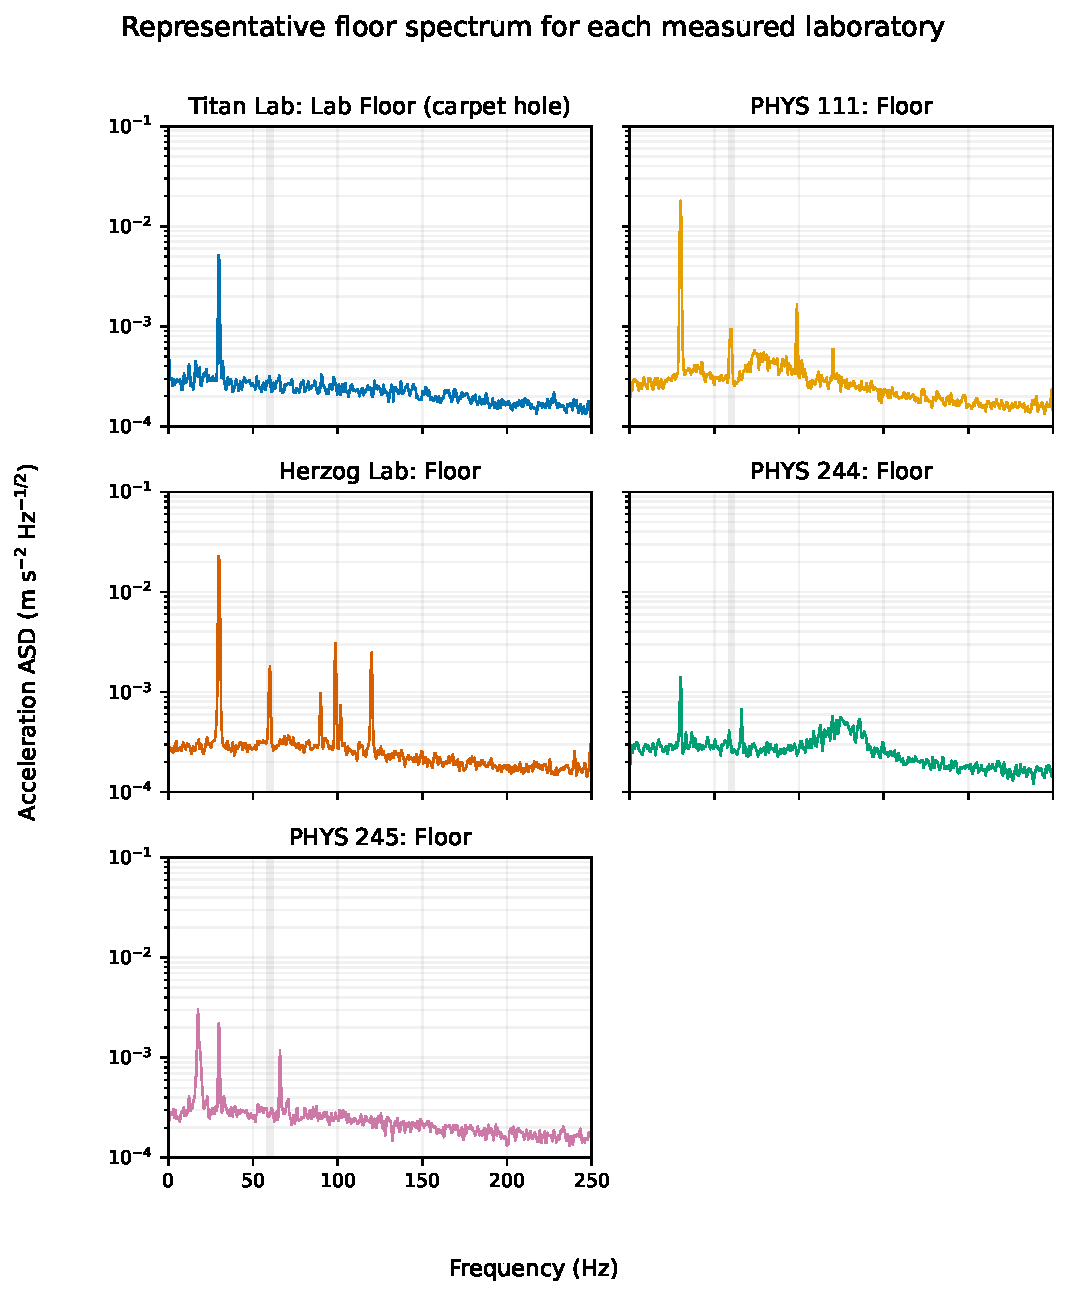
\includegraphics[height=0.82\textheight,keepaspectratio]{representative_spectra_by_room.pdf}
\caption{Representative floor spectra, shown separately with common axes. The
gray band is the excluded \freqrange{58}{62} mains region. This is the
same floor-by-floor presentation used in the full report.}
\label{fig:floor-panels}
\end{figure}

The broad noise floors are similar, particularly at higher frequencies.
Room selection is therefore driven mainly by the discrete peaks. The
integrated values in Figure~\ref{fig:rms-context} demonstrate why a simple RMS
ranking can be misleading: Titan's \freq{29.8} line raises its total,
even though the background between peaks is the lowest of the candidate rooms.

\begin{figure}[H]
\centering
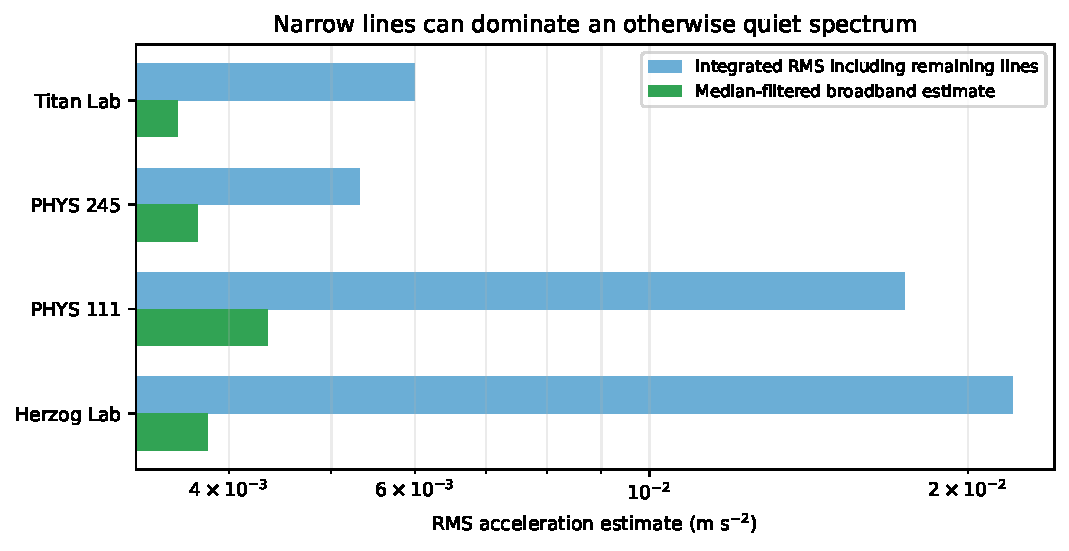
\includegraphics[width=0.92\linewidth]{candidate_rms_context.pdf}
\caption{Integrated RMS including the remaining narrow lines compared with a
median-filtered estimate of the broadband background. The PHYS 111 and Herzog
integrated values use the conservative freezer adjustment described below.}
\label{fig:rms-context}
\end{figure}

\begin{table}[H]
\centering
\caption{Peak-centered comparison of the candidate floor measurements.
RMS values are in $10^{-3}$ \si{\meter\per\second\squared}; peak ASD values
are in $10^{-3}$ \asdunit.}
\begin{tabular}{lrrrr}
\toprule
Room & Integrated RMS & Background estimate & Largest peak & Peak ASD\\
\midrule
Titan Lab  & 5.99 & 3.58 & 29.8 Hz & 5.15\\
PHYS 245   & 5.31 & 3.74 & 17.6 Hz & 3.07\\
PHYS 111   & 17.4 & 4.35 & 29.8 Hz & 18.0\\
Herzog Lab & 22.0 & 3.81 & 29.8 Hz & 22.9\\
\bottomrule
\end{tabular}
\end{table}

\subsection{PHYS 245 and its neighboring room}

The PHYS 245 and PHYS 244 floor measurements are similar in broadband level,
which is reasonable given their proximity. PHYS 245 actually has the slightly
lower median-filtered background estimate
(\SI{3.74e-3}{\meter\per\second\squared} versus
\SI{4.18e-3}{\meter\per\second\squared}), but the rooms are not spectrally
identical. PHYS 245 has stronger narrow lines near 17.6, 29.8, and 66.0 Hz.

\section{Optical-table performance}

\begin{figure}[H]
\centering
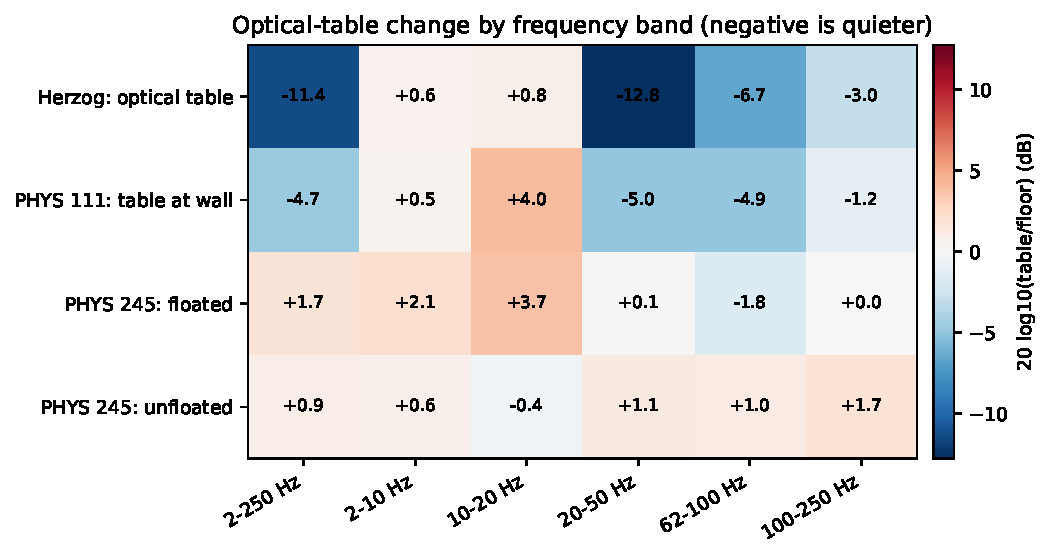
\includegraphics[width=0.94\linewidth]{optical_table_performance.pdf}
\caption{Band-limited change from floor to table. Negative values are
attenuation; positive values are amplification.}
\label{fig:tables}
\end{figure}

The plot carries the main conclusion. The Herzog optical-table measurement is
substantially quieter above \freq{20}, and the PHYS 111 table at the
Herzog wall also improves the higher-frequency bands. The explicitly floated
PHYS 245 table does not improve the supplied run overall and is worse from
\freqrange{10}{20}; its isolators and loading should be checked before
that result is treated as representative.

\section{Herzog, PHYS 111, and the freezer}

\begin{figure}[H]
\centering
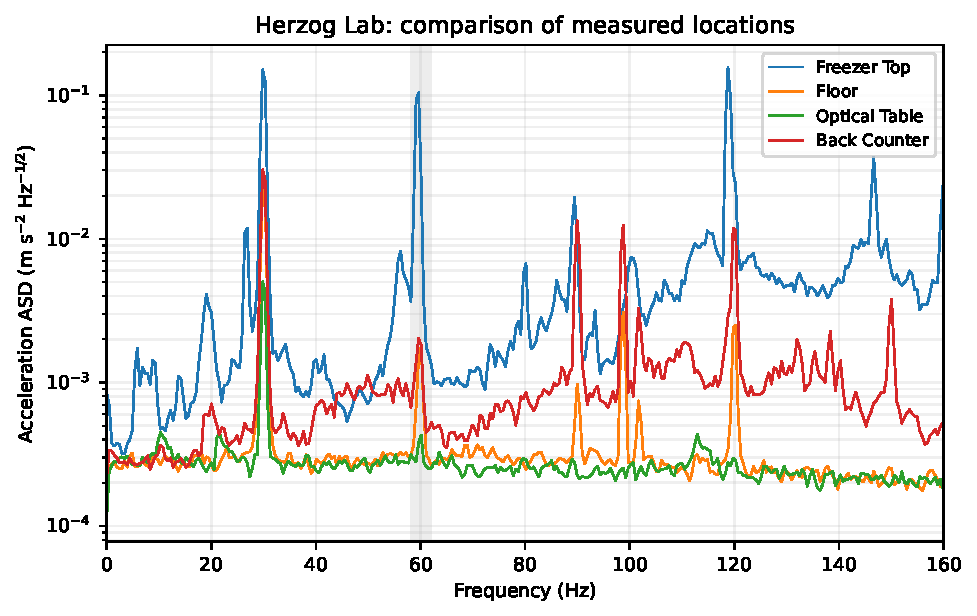
\includegraphics[width=0.94\linewidth]{within_herzog_lab.pdf}
\caption{The measured locations in Herzog. The freezer-top run is a source
reference, not a candidate experimental location.}
\label{fig:herzog-room}
\end{figure}

The spectra measured on the freezer and on the Herzog floor are used as a
source-reference pair. Peaks are matched using only the numerical ASD data.
A matched line is treated as freezer-specific only when it is not also present
on at least two distant floor spectra. This identifies a Herzog feature near
\freq{89.9} that matches the freezer near \freq{89.4}, and a
Herzog/PHYS 111 feature near \freq{120.2} that matches the freezer's
strong cluster near \freq{118.8}.

The \freq{29.8} line is strong on the freezer, but it is also present on
all distant floors. It is therefore retained rather than attributed to the
freezer.

\section{Why Titan is preferred}

\begin{figure}[H]
\centering
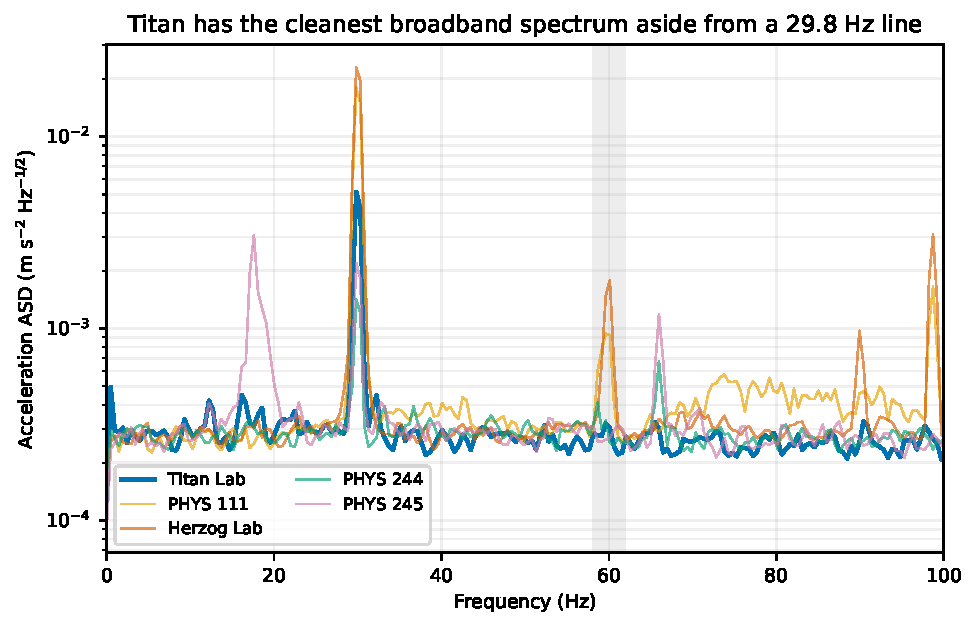
\includegraphics[width=0.94\linewidth]{titan_vs_other_floors.pdf}
\caption{Titan compared with the representative floor spectra. Titan has the
lowest broadband background and the fewest prominent non-mains lines. Its
\freq{29.8} feature remains important for experiments with a mechanical
response near that frequency.}
\label{fig:titan}
\end{figure}

Figure~\ref{fig:titan} is the clearest practical summary. Titan stays at or
below the other candidate spectra through most of the displayed range.
Its one important qualification is the narrow \freq{29.8} line. For
spectroscopy, a floated and well-tuned table in Titan should therefore be the
first configuration tested.

\section{Freezer-informed adjustment}

\begin{figure}[H]
\centering
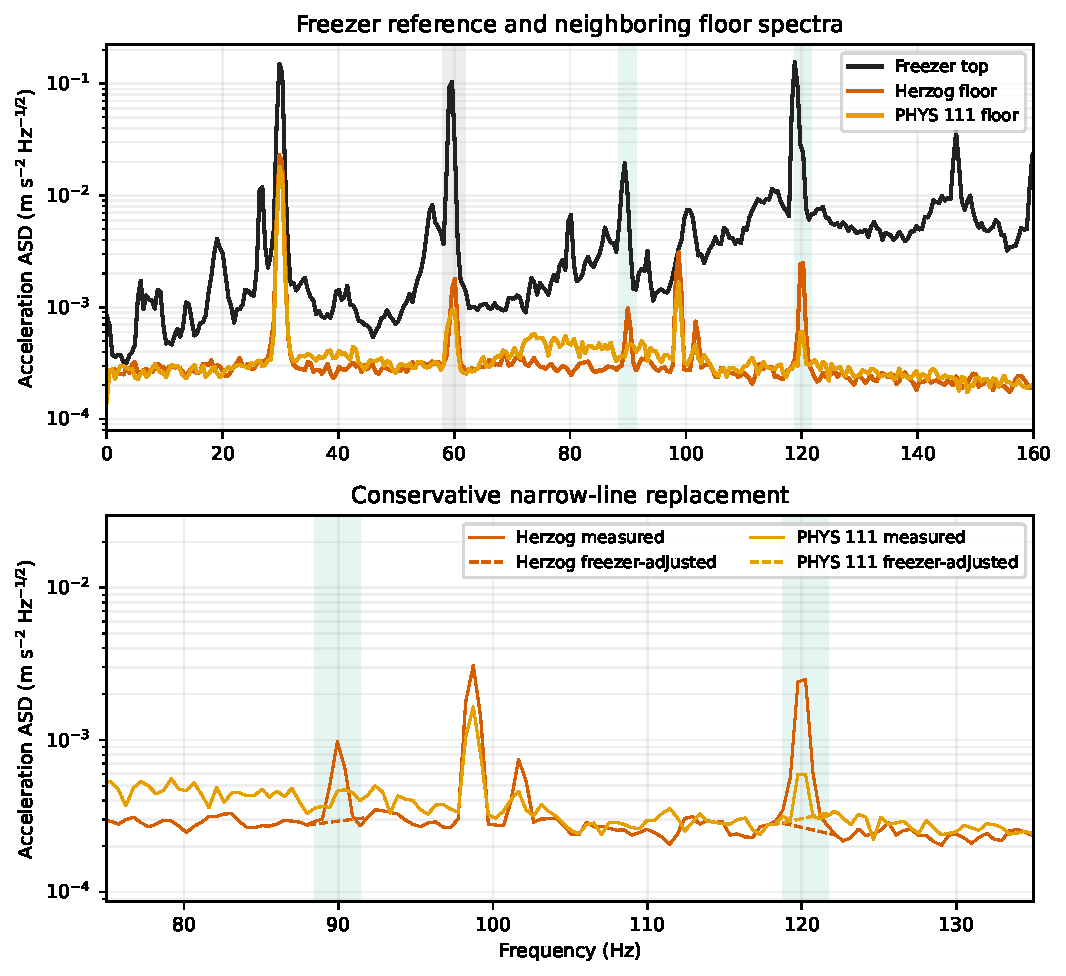
\includegraphics[width=0.94\linewidth]{freezer_informed_adjustment.pdf}
\caption{Top: the freezer reference with the Herzog and PHYS 111 floors.
Bottom: measured and freezer-adjusted floor spectra. Green bands mark the
narrow lines replaced in at least one room; the gray band marks the excluded
mains region.}
\label{fig:freezer-adjustment}
\end{figure}

The adjustment does not subtract the freezer ASD directly. The measurements
were not simultaneous, and no phase or transfer function is available, so
direct amplitude subtraction would not be defensible. Instead, only the
source-specific matched lines are replaced over a narrow
$\pm$\freq{1.5} interval by a log-linear interpolation of the local
floor background.

This adjustment lowers the Herzog integrated RMS from
\SI{2.220e-2}{\meter\per\second\squared} to
\SI{2.204e-2}{\meter\per\second\squared}; the PHYS 111 value changes from
\SI{1.741e-2}{\meter\per\second\squared} to
\SI{1.741e-2}{\meter\per\second\squared} at the shown precision. The small
change confirms that the freezer-specific lines are real but are not the main
reason these rooms compare poorly. The retained \freq{29.8} line is the
dominant difference.

\section{The 60 Hz feature}

\begin{figure}[H]
\centering
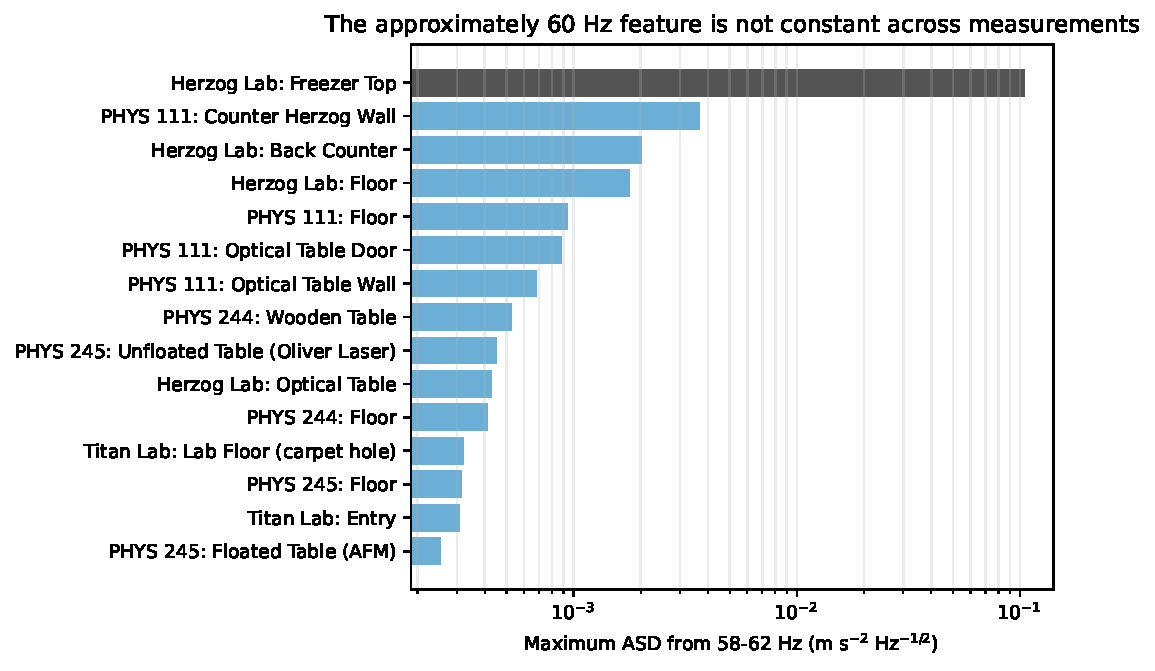
\includegraphics[width=0.94\linewidth]{sixty_hz_feature_comparison.pdf}
\caption{Maximum ASD within the excluded \freqrange{58}{62} band. The
line appears everywhere but varies substantially in amplitude.}
\label{fig:mains}
\end{figure}

The universal narrow line is consistent with electrical mains coupling into
the sensor or acquisition electronics. Its large run-to-run variation,
especially on the freezer and surfaces near Herzog, suggests that the measured
feature is not a perfectly constant electronic offset. It may contain a
mechanical component or equipment-dependent electrical coupling. Either way,
it is not used to rank the rooms.

\section{Practical conclusion}

\begin{enumerate}
  \item \textbf{Titan Lab} is the preferred room for spectroscopic work because
        it has the lowest broadband background and the simplest peak structure.
  \item \textbf{PHYS 245} is the best alternative. Its broadband level is close
        to Titan, but its 17.6, 29.8, and 66.0 Hz lines deserve attention.
  \item \textbf{PHYS 111 and Herzog} have much stronger 29.8 Hz motion.
        Freezer-specific correction does not change that conclusion.
  \item Use a floated table, but verify that it is actually floating and
        correctly loaded. The supplied PHYS 245 floated-table run shows that
        an isolation system can perform poorly near its resonance.
  \item Before final installation, repeat simultaneous floor/table
        measurements in Titan and PHYS 245, and repeat the Herzog/PHYS 111
        measurements with the freezer compressor deliberately on and off.
\end{enumerate}

The measurements support a clear room choice, but they do not identify the
neighboring turbine as a unique source. A synchronized on/off test would be
required for that attribution.

\end{document}
